\documentclass[10pt,letterpaper]{article} 
%\usepackage{tikz}
\usepackage{amsmath,amssymb,geometry,caption,subcaption}
%\usepackage{graphicx}‎‎
%\usefonttheme{serif}‎
%\usepackage{ptext}‎
\usepackage{xepersian}
%\settextfont{B Nazanin}
\usepackage{lipsum}
\setlength{\parindent}{0pt}
%\usepackage{enumitem}
%\setlist[enumerate,1]{label=(\arabic*)}
\newcommand{\pf}{$\blacksquare$}
\newcommand{\EX}{\Bbb E}
\newcommand{\nl}{\newline\newline}
\setlength{\parskip}{1em}

\usepackage{amsmath}
\usepackage{accents}
\newlength{\dhatheight}
\newcommand{\doublehat}[1]{%
    \settoheight{\dhatheight}{\ensuremath{\hat{#1}}}%
    \addtolength{\dhatheight}{-0.35ex}%
    \hat{\vphantom{\rule{1pt}{\dhatheight}}%
    \smash{\hat{#1}}}}

\newcounter{QuestionNumber}
\setcounter{QuestionNumber}{1}

\newcommand{\Q}{
\textbf{
سوال \theQuestionNumber)
}
\stepcounter{QuestionNumber}
}

\newcommand{\fig}[3]{
\begin{figure}[h!]
#1
\caption{#2}
\label{#3}
\end{figure}
}

\newcommand{\subfig}[3]{
\begin{subfigure}{#3}
#1
\caption{#2}
\end{subfigure}
}
%\newcommand{\pic}[2]{
%\begin{center}
%\includegraphics[width=#2]{#1}
%\end{center}
%}
\begin{document}
\Large
\begin{center}
به نام زیبایی

تمرینات سری یازدهم سیگنال ها و سیستم ها

\hrulefill
\end{center}
%\Q
%
%تبدیل فوریه‌ی سیگنال های زمان گسسته‌ی زیر را به دست آورید.
%
%الف)
%$
%x[n]=u[n]-u[n-5]
%$
%
%ب)
%$
%x[n]=({1\over 3})^nu[n]
%$
%
%پ)
%$
%x[n]=-({1\over 3})^nu[-n-1]
%$
%
%ت)
%$
%x[n]=\sin{\pi\over 2}n+\cos n
%$
%
%ث) 
%$
%x[n]=n({1\over 3})^nu[n]
%$
%
%\Q
%
%عکس تبدیل فوریه‌ی سیگنال های زیر را به دست آورید.
%
%الف)
%$
%X(e^{j\omega})=\sum_{k=-\infty}^{\infty}(-1)^k\delta(\omega-{\pi\over 2}k)
%$
%
%ب)
%$
%X(e^{j\omega})={1-{1\over 3}e^{-j\omega}\over 1-{1\over 4}e^{-j\omega}-{1\over 8}e^{-2j\omega}}
%$
%
%پ) 
%$
%X(e^{j\omega})={1\over 1-e^{-4j\omega}}
%$

\large

\Q

تبدیل z سیگنالهای زیر را به همراه ناحیه همگرایی آن به دست آورید.

الف)
$
x[n]=(-\frac{1}{2})^n\sin 2nu[n]
$

ب) 
$
x[n]=\frac{1}{n}(\frac{1}{2})^n
$

پ)
$
x[n]=(-1)^nu[n]+\alpha^n u[-n-1]
$
که $\alpha$ یک مقدار حقیقی است.

ت)
$
x[n]=(\frac{1}{2})^n\{u[n+3]-u[n-2]\}
$

\Q

عکس تبدیل z هر یک از موارد زیر را بیابید.

الف)
$
X(z)=\frac{1-\frac{1}{2}z^{-1}}{(1-\frac{1}{3}z^{-1})(1+\frac{1}{4}z^{-2})}
\quad,\quad \text{ROC}=\{\frac{1}{3}<|z|<\frac{1}{2}\}
$

ب)
$
X(z)=\frac{1}{(1-\frac{1}{2}z^{-1})(1-2z^{-1}+\frac{15}{16}z^{-2})}
\quad,\quad \text{ROC}=\{|z|<\frac{1}{2}\}
$

\Q

سیگنال 
$
x[n]=(\frac{1}{3})^nu[n]+(-\frac{1}{3})^nu[n]
$
به سیستمی پایدار با تبدیل z پاسخ ضربه 
$
H(z)=\frac{1-\frac{1}{3}z^{-1}}{(1-\frac{1}{2}z^{-1})(1-2z^{-1})^2}
$
وارد می‌شود. خروجی این سیستم را بیابید.

\Q

نمودار صفر-قطب پاسخ ضربه‌ی دو سیستم گسسته‌ (سیستم 1 با پاسخ ضربه‌ی 
$
h_1[n]
$
و سیستم 2 با پاسخ ضربه‌ی 
$
h_2[n]
$
)
 به صورت زیر است:
\begin{figure}[h!]
\centering
\begin{subfigure}{0.49\textwidth}
\includegraphics[width=70mm]{PS12_Q3_6.eps}
\caption{
نمودار صفر-قطب سیستم 1؛ این سیستم دارای دو قطب در $0.8$ و $1.2$ و دو صفر در $0.3$ و $-1$ است.
}
\end{subfigure}
\begin{subfigure}{0.49\textwidth}
\includegraphics[width=70mm]{PS12_Q3_5.eps}
\caption{
نمودار صفر-قطب سیستم 2
}
\end{subfigure}
\end{figure}

سیستم 1 پایدار و سیستم 2 علی است.

الف) آیا سیستم 1 علی است؟ دوطرفه چطور؟

ب) آیا سیستم 2 پایدار است؟

پ) پاسخ فرکانسی سیستم 1 ($H_1(e^{j\omega})$) در کدام فرکانس صفر می شود؟

ت) نمودار صفر-قطب تبدیل z سیستم معکوس سیستم 1 را رسم و ناحیه همگرایی آن را تعیین کنید.

ث) (امتیازی) با رسم تقریبی اندازه‌ی پاسخ فرکانسی سیستم 1 ($|H_1(e^{j\omega})|$) استدلال کنید این سیستم فیلتر بالاگذر است یا میان گذر یا پایین گذر.

\Q

نمودار صفر-قطب تبدیل z یک سیستم LTI به صورت زیر است:

\begin{figure}[h!]
\centering
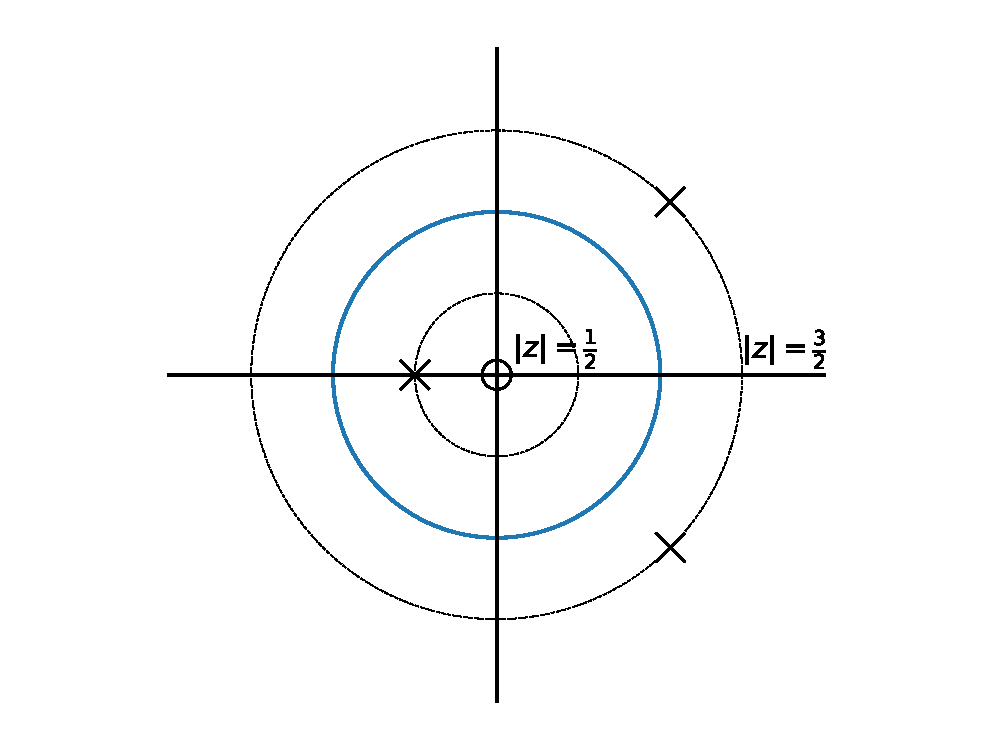
\includegraphics[width=90mm]{i1.eps}
\end{figure}
که قطب های مختلط دارای زاویه‌ی 
$
\pm 45^\circ
$
هستند. پاسخ ضربه سیستم را در حالتی که 

الف) پایدار باشد

ب) علی و ناپایدار باشد

پ) ضدعلی باشد

به دست آورید.

\Q

سیستم حقیقی، زمان گسسته و پایدار $h[n]$ با تبدیل $z$ زیر توصیف می شود:
$$
H(z)={1-az^{-1}\over (1-2z^{-1})\left(1-{1\over 2}z^{-1}\right)}
$$

الف) آیا می توان با تغییر مقادیر $a$، سیستم را علی نمود؟ ضد-علی چطور؟

ب) محدوده‌ی مقادیری از $a$ را بیابید که سیستم، وارون علی و پایدار داشته باشد.

پ) نمودار صفر و قطب سیستم وارون را رسم کنید.

\Q

یک سیستم LTI با پاسخ ضربه 
$
h[n]
$
که تبدیل z آن، تابع کسری
$
H(z)
$
است، دارای خواص زیر است:
\begin{itemize}
\item
$
h[n]
$
حقیقی است.
\item
$
H(z)
$
دارای دو قطب محدود و یک صفر در $z=3$ است.
\item
یکی از قطب ها در 
$
z=2
$
قرار دارد.
\item
پاسخ این سیستم به ورودی های 
$
(\frac{3}{2})^n
$
و
$
(\frac{4}{3})^n
$
به ترتیب برابر 
$
4(\frac{3}{2})^{n+2}
$
و
$
10(\frac{4}{3})^n
$
است.
\end{itemize}
در این صورت

الف) نمودار صفر-قطب سیستم را رسم کنید.

ب) پاسخ سیستم را به ورودی 
$
x[n]=(-\frac{1}{4})^{n}
$
بیابید.

پ) پاسخ ضربه سیستم معکوس را بیابید.
\end{document}